\section{Address Malleability}\label{subsec:malleability_predicate}

We first introduce the notion of address malleability. We describe the
adversarial threat models that might exploit it, distill the components that
define a malleability attack, and organize this family of attacks based on
threat levels. Next, we formalize malleability via the \emph{malleability
predicate} and present a formal addressing of these attacks. Before proceeding
with the definition though, we first define the objects that underpin our
constructions and explore the malleability of addresses.

An \emph{account} comprises of multiple addresses.  An address is associated
with a number $\addrgenlength$ of \emph{attributes}, each identifying a
property of the address, which are organized as follows:
\begin{inparaenum}[i)]
    \item \emph{public} attributes are part of the address, so they are public
        and available without any interaction with the account's owner;
    \item \emph{semi-public} attributes are not public by default, but become
        public when a transaction is issued, which spends some assets that the
        address owns;
    \item \emph{private} attributes never become public.
\end{inparaenum}
An \emph{attribute list} $l$ is a vector of $\addrgenlength$ attributes. In our
work, the fundamental list of attributes is the \emph{address generation list}
$\addressgenlist$, \ie the list of all attributes used during the generation of
an address $\addr$. In this list, the sub-list of public attributes $d =
(\attribute_1, \ldots, \attribute_{p-1})$ contains the attributes which are
available by every party with access to the address. Of the remaining
attributes, the sub-list $(\attribute_p, \ldots, \attribute_{i-1})$ contains
the semi-public attributes, while $(\attribute_i, \ldots,
\attribute_\addrgenlength)$ contains the private attributes. The parameters $p$
and $i$ depend on the inner workings of the protocol and the address generation
scheme. For example, in Bitcoin, a typical address attribute is the payment key
pair $\paymentkeypair$: $\paymentkeyverify$ is used to verify signatures and is
\emph{semi-public}, its hash is a \emph{public} attribute, whereas
$\paymentkeysign$, which signs transactions, is \emph{private}.

Before exploring address malleability, a brief motivation is necessary. Address
malleability is similar to the preexisting malleability
notions~\cite{dolev2003nonmalleable} and is intrinsically tied to address
generation. Here, we treat it as a novel family of attack vectors due to the
complex structure of PoS addresses. Namely, our framework's addresses encode
information that extend beyond the simple transfer of assets and pertain to
additional functionalities, like staking. Therefore, to ensure the PoS
protocol's security, it is crucial to prevent an adversary $\adversary$ from
constructing addresses on behalf of honest users, or manipulating honestly
generated addresses.

The goal of $\adversary$ is to inflate their stake in the system by exploiting
address malleability. We remind that an address is associated with the payment
information $\accPay$, which is used to issue payments (and practically
controls the assets) and the staking information $\accSta$, which is used to
participate in the PoS consensus protocol. $\adversary$ attempts to forge an
address, for which it controls the staking information $\accSta$ without
controlling the payment information $\accPay$. This results in a stake
``shift'', via which $\adversary$ gains illegitimate control of the staking
rights of assets it does not own.  Importantly, this forgery should take place
in such a way that the address's honest owner does not easily recognize this
stake shift, unless actively looking for it.

Numerous types of adversaries would try to exploit this hazard.  One such type
is a malicious stake pool leader. Such attacker would operate under the ---
natural --- assumption that the reward amount depends on the stake percentage,
the staking rights of which the pool controls. This assumption is amplified
given incentives mechanisms~\cite{DBLP:journals/corr/abs-1807-11218} which
mandate that larger stake pools receive greater rewards. By deploying a
generalized malleability attack, $\adversary$ would artificially increase the
amount of its rewards (Figure~\ref{fig:malleability_attack}). To deploy this
attack, $\adversary$ could intercept honestly-generated addresses, which are
exchanged between users, and replace them with forged addresses which are
created on-the-fly. As long as $\adversary$ remains unnoticed, it may be very
profitable to mount such attack on a broad network level.

\begin{figure}
  \begin{center}
    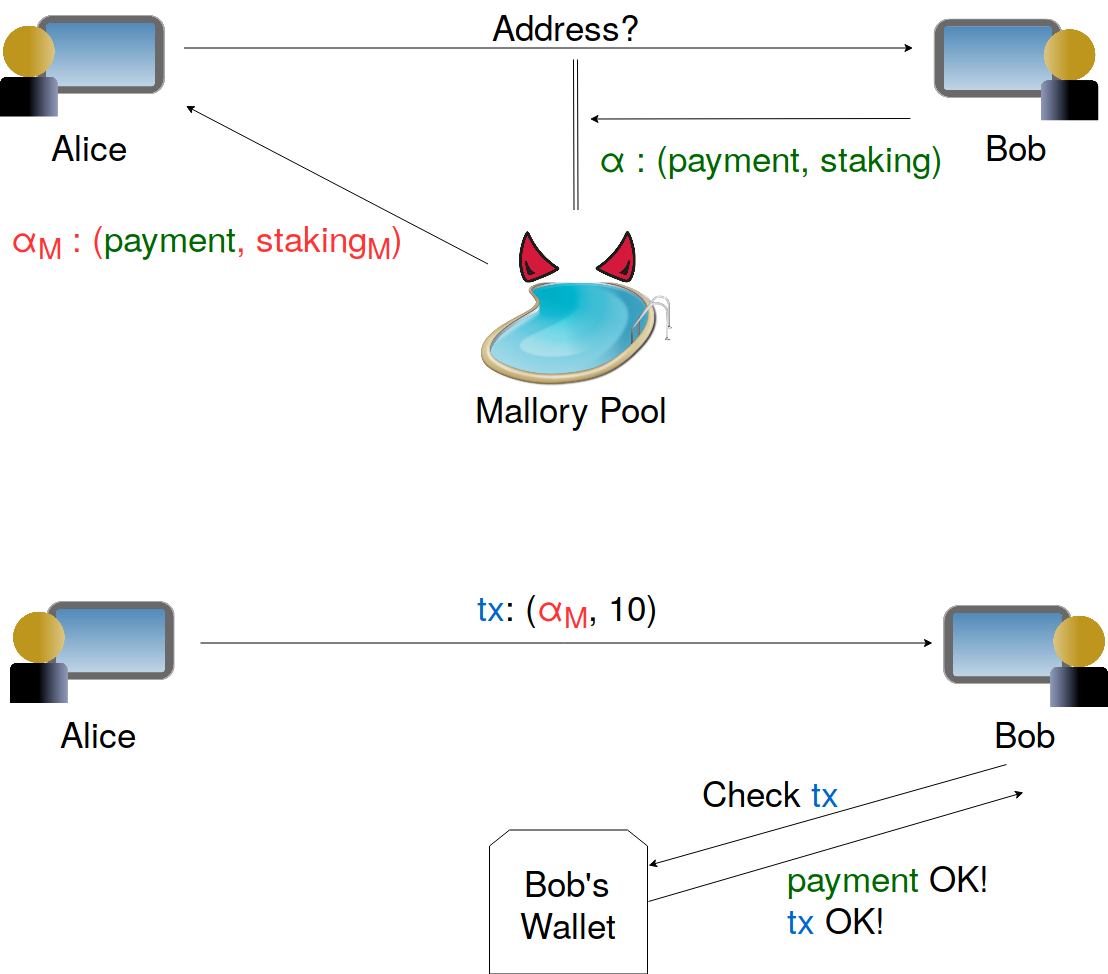
\includegraphics[width=0.6\textwidth]{figures/delegation/malleability_attack.png}
  \end{center}
  \caption{
      An example of a network-level, Man-in-the-Middle malleability attack. A
      malicious pool changes on-the-fly the staking object of one of Bob's
      addresses, such that it points to Mallory's stake pool. If Bob's wallet
      does not identify the attack, Mallory has successfully (but artificially)
      inflated its delegated stake. If the wallet does identify the attack, it
      has to transfer the funds to a correct address and impose extra fees on
      Bob.
    }
  \label{fig:malleability_attack}
\end{figure}

Following we identify multiple types of address malleability attacks. In all
cases, we assume that the adversary does not control the signing payment key
$\paymentkeysign$, as this would trivialize all attacks. An address created by
$\adversary$ without access to its payment key is called \emph{forgery}. A
forgery is successful if funds that are sent to it can be spent and the wallet
accepts the forged address as its own, whereas it fails if funds that are sent
to it can never be spent and are, therefore, ``burnt''.

Our analysis assumes two types of adversaries, depending on the level of
information which they access. First is the \emph{network adversary}, who has
access to the ledger, observes the network, and can intercept addresses
exchanged between parties. Second is the \emph{targeting adversary}, with
access to the same information as the first, but also knows the set of past
transactions issued by the ``victim'', \ie the honest user for which it
attempts to produce a forgery. We stress that the assumptions for the targeting
adversary are much stronger compared to the network adversary.

The malleability levels presented next range from \emph{full malleability}, \ie
when no inherent protection against malleability attacks exists, to \emph{non
malleability}, \ie where an adversary cannot create a successful forgery
without access to the address's private attributes. Defining the intermediate
levels allows us to construct various address schemes, which are suitable for
different needs of real world projects.  For example, a fully malleable address
is typically short and suitable for performance-oriented applications.  In
contrast, a security-oriented project would aim for the higher levels of
malleability protection. The malleability levels are organized around the
following three properties:
\begin{inparaenum}[i)]
    \item the type of adversary, \ie $\adversary$ is at the network level or
        has targeted access to the user's wallet;
    \item self-verification, \ie whether a wallet can recognize a forgery
        for one of its own payment keys;
    \item cross-verification, \ie whether a wallet can identify a forgery
        for an address which it does not own.
\end{inparaenum}
Below we describe the malleability levels and summarize them in
Table~\ref{tab:malleability_levels}:
\begin{itemize}
    \item \emph{Level 1, Full Malleability:} This level enables successful
        forgeries from both network and targeting adversaries. A wallet checks
        only the payment information, so it accepts the forgery without
        recognizing it as such, while also both spending from and sending funds
        to forgeries.
    \item \emph{Level 2, Full Verifiable Malleability:} Again, both types of
        adversaries, \ie network and targeting, can create forgeries. However,
        during recovery, the wallet identifies forgeries and rejects them; we
        note that a ``hacked'' wallet can spend the assets
        owned by such forgery. Also all wallets, including honest ones, may
        send funds to forgeries.
    \item \emph{Level 3, A Posteriori Malleability:} This level prohibits
        network adversaries. Specifically, if such adversary produces a
        forgery, any transaction which spends from the forgery is rejected.
        However, targeting adversaries can create successful forgeries as
        before.
    \item \emph{Level 4, A Posteriori Verifiable Malleability:} This level is
        similar to \emph{Level 3}, with the addition that an honest wallet can
        identify and reject forgeries of its own addresses, as in \emph{Level
        2}.
    \item \emph{Level 5, ``Sink'' Malleability:} Both network and targeting
        adversaries are prohibited. Thus, all forgeries are rejected by the
        wallet and its funds are burnt. Intuitively, considering
        transactions as a graph, where the graph's nodes are the addresses and
        its edges are transactions, forgeries are ``sinks'' which trap all
        funds sent to them. However, a wallet still cannot identify a forgery
        of an address that it does not own.
    \item \emph{Level 6, Non Malleability:} The highest level of
        protection against malleability, where a forgery is rejected by every
        wallet, \ie given only an address anybody can identify whether it is
        honestly-generated or a forgery. Therefore, all transactions that
        interact in any way with a forgery are rejected.
\end{itemize}

\begin{table}[]
\centering \def\arraystretch{1.5}

\begin{center}
  \begin{tabular}{|c|c|c|c|c|}
    \cline{1-5}
          \multicolumn{1}{|c|}{\begin{tabular}[c]{@{}c@{}} Level of \\ Malleability \end{tabular}}
        & \multicolumn{1}{c|}{\begin{tabular}[c]{@{}c@{}} Network \\ protection \end{tabular}}
        & \multicolumn{1}{c|}{\begin{tabular}[c]{@{}c@{}} Targeting \\ protection \end{tabular}}
        & \multicolumn{1}{c|}{\begin{tabular}[c]{@{}c@{}} Self-\\verification \end{tabular}}
        & \multicolumn{1}{c|}{\begin{tabular}[c]{@{}c@{}} Cross-\\verification \end{tabular}} \\
    \hline
       \multicolumn{1}{|l|}{\begin{tabular}[c]{@{}c@{}} 1 - Full \end{tabular}}
     & \multicolumn{1}{c|}{\begin{tabular}[c]{@{}c@{}} \xmark \end{tabular}}
     & \multicolumn{1}{c|}{\begin{tabular}[c]{@{}c@{}} \xmark \end{tabular}}
     & \multicolumn{1}{c|}{\begin{tabular}[c]{@{}c@{}} \xmark \end{tabular}}
     & \multicolumn{1}{c|}{\begin{tabular}[c]{@{}c@{}} \xmark \end{tabular}} \\
    \hline
       \multicolumn{1}{|l|}{\begin{tabular}[c]{@{}c@{}} 2 - Verifiable  \end{tabular}}
     & \multicolumn{1}{c|}{\begin{tabular}[c]{@{}c@{}} \xmark \end{tabular}}
     & \multicolumn{1}{c|}{\begin{tabular}[c]{@{}c@{}} \xmark \end{tabular}}
     & \multicolumn{1}{c|}{\begin{tabular}[c]{@{}c@{}} \cmark \end{tabular}}
     & \multicolumn{1}{c|}{\begin{tabular}[c]{@{}c@{}} \xmark \end{tabular}} \\
    \hline
       \multicolumn{1}{|l|}{\begin{tabular}[c]{@{}c@{}} 3 - A posteriori  \end{tabular}}
     & \multicolumn{1}{c|}{\begin{tabular}[c]{@{}c@{}} \cmark \end{tabular}}
     & \multicolumn{1}{c|}{\begin{tabular}[c]{@{}c@{}} \xmark \end{tabular}}
     & \multicolumn{1}{c|}{\begin{tabular}[c]{@{}c@{}} \xmark \end{tabular}}
     & \multicolumn{1}{c|}{\begin{tabular}[c]{@{}c@{}} \xmark \end{tabular}} \\
    \hline
       \multicolumn{1}{|l|}{\begin{tabular}[c]{@{}c@{}} 4 - A posteriori \\ verifiable  \end{tabular}}
     & \multicolumn{1}{c|}{\begin{tabular}[c]{@{}c@{}} \cmark \end{tabular}}
     & \multicolumn{1}{c|}{\begin{tabular}[c]{@{}c@{}} \xmark \end{tabular}}
     & \multicolumn{1}{c|}{\begin{tabular}[c]{@{}c@{}} \cmark \end{tabular}}
     & \multicolumn{1}{c|}{\begin{tabular}[c]{@{}c@{}} \xmark \end{tabular}} \\
    \hline
       \multicolumn{1}{|l|}{\begin{tabular}[c]{@{}c@{}} 5 - Sink  \end{tabular}}
     & \multicolumn{1}{c|}{\begin{tabular}[c]{@{}c@{}} \cmark \end{tabular}}
     & \multicolumn{1}{c|}{\begin{tabular}[c]{@{}c@{}} \cmark \end{tabular}}
     & \multicolumn{1}{c|}{\begin{tabular}[c]{@{}c@{}} \cmark \end{tabular}}
     & \multicolumn{1}{c|}{\begin{tabular}[c]{@{}c@{}} \xmark \end{tabular}} \\
    \hline
       \multicolumn{1}{|l|}{\begin{tabular}[c]{@{}c@{}} 6 - None  \end{tabular}}
     & \multicolumn{1}{c|}{\begin{tabular}[c]{@{}c@{}} \cmark \end{tabular}}
     & \multicolumn{1}{c|}{\begin{tabular}[c]{@{}c@{}} \cmark \end{tabular}}
     & \multicolumn{1}{c|}{\begin{tabular}[c]{@{}c@{}} \cmark \end{tabular}}
     & \multicolumn{1}{c|}{\begin{tabular}[c]{@{}c@{}} \cmark \end{tabular}} \\
    \hline
  \end{tabular}
\end{center}
\normalsize
\caption{Comparison of the malleability levels.}\label{tab:malleability_levels}
\end{table}

We now formalize address malleability with the predicate $M$. The predicate
returns $1$ or $0$ to denote whether an address is valid or not.  Here, a valid
address is either honestly-generated or a successful forgery, \ie it is an
address that the wallet accepts. The first parameter of the predicate is the
set $L_{\party}$ of all created addresses and their attributes for a party
$\party$; this parameter is necessary, so that the predicate compares the given
address with the honestly generated ones. The second parameter is the auxiliary
information $\msf{aux}_M$, which takes the values $\msf{recover}$ $\msf{issue}$ or
$\msf{verify}$ this information is used to instantiate different modes of the
predicate and allows it to adjust its actions, thus making it more versatile.
The third parameter is the address under question.

\paragraph{Full Malleability}
This predicate does not allow the ideal functionality to perform any
malleability checks when issuing a transaction. During recovery and
verification, it first identifies the list of public attributes $d$, then
outputs $1$ if these attributes have been used in at least one address that the
wallet controls. Intuitively, a forgery can be constructed by using public
attributes from other addresses that the wallet has created. In the real-world,
the wallet accepts an address as long as its payment key is controlled by the
wallet. In a \emph{fully malleable} construction, the predicate is instantiated
with $M_{\mathsf{FM}}$ described in Algorithm \ref{algo:fm_predicate}; the
function $\mathrm{parsePubAttrs}$ denotes the public attribute parsing  of an
address.

\begin{algorithm}
    \caption{The \emph{fully malleable} predicate. The inputs are: i) a list of tuples of previously-generated addresses and their attributes, ii) auxiliary information on the wallet's operation, iii) the address under question.}\label{algo:fm_predicate}
    \begin{algorithmic}
        \Function{$M_{\mathsf{FM}}$}{$L_P, \msf{aux}_M, \addr$}
            \Switch{$\msf{aux}_M$}
                \Case{$\msf{issue}$}
                    \State \Return 1
                \EndCase
                \Case{$\msf{verify}$ OR $\msf{recover}$}
                    \State $d = \textrm{parsePubAttrs}(\addr)$
                    \For {$\attribute \in d$}
                        \If {$\forall \addr' \in L_P, d' = \textrm{parsePubAttrs}(\addr')$: $\attribute \not \in d'$}
                            \State \Return 0 \Comment{$\attribute$ not registered detected}
                        \EndIf
                    \EndFor
                \EndCase
            \EndSwitch
            \State \Return 1
        \EndFunction
    \end{algorithmic}
\end{algorithm}

\paragraph{A Posteriori Malleability}
In an \emph{a posteriori malleable} construction, the predicate first
identifies the list $d$ of public attributes of the address $\addr$.  Then, for
each such attribute $\attribute$, it checks:
\begin{inparaenum}[i)]
    \item if there exists an issued transaction $\tx = (\assetset, \addr_s,
        \addr_r, m)$, such that the public attributes of $\addr_s$ include
        $\attribute$;
    \item if there exists an address that the wallet has created, such that
        $\attribute$ is part of its public attributes.
\end{inparaenum}
If both checks fail the predicate returns $0$, otherwise $1$.  Intuitively,
this construction enables malleability only for addresses whose payment key has
been previously used and for which all public attributes have been used in
other addresses. Therefore, as long as the payment key of the address has not
been used, the scheme provides non-malleability. The \emph{a posteriori
malleable} construction, instantiated with the predicate
$M^{\mathbb{T}}_{\mathsf{PM}}$ which is parameterized by the list of all
transactions $\mathbb{T}$, is described in Algorithm \ref{algo:pm_predicate}.

\begin{algorithm}
    \caption{The \emph{a posteriori} malleability predicate. The inputs are: i) a list of tuples of previously-generated addresses and their attributes, ii) auxiliary information on the wallet's operation, iii) the address under question.}\label{algo:pm_predicate}
    \begin{algorithmic}
        \Function {$M^{\mathbb{T}}_{\mathsf{PM}}$}{$L_P, \msf{aux}_M, \addr$}
            \Switch{$\msf{aux}_M$}
                \Case{$\msf{issue}$}
                    \State \Return 1
                \EndCase
                \Case{$\msf{verify}$ OR $\msf{recover}$}
                    \State $d = \textrm{parsePubAttrs}(\addr)$
                    \For {$\attribute \in d$}
                        \If {$\forall \addr' \in L_P, d' = \textrm{parsePubAttrs}(\addr')$: $\attribute \not \in d'$}
                            \State \Return 0
                        \EndIf
                        \If {$\forall (\assetset, \addr_s, \addr_r, m) \in \mathbb{T}, d_s = \textrm{parsePubAttrs}(\addr_s)$: $\attribute \not \in d_s$}
                            \State \Return 0
                        \EndIf
                    \EndFor
                    \State \Return 1
                \EndCase
            \EndSwitch
        \EndFunction
    \end{algorithmic}
\end{algorithm}

\paragraph{Sink Malleability}
Intuitively, a \emph{sink malleable} address generation algorithm requires that
only the owner of the honest wallet can create addresses for payment keys of
the wallet. This is expressed by differentiating the behavior depending on the
auxiliary information. If $\msf{aux}_M$ pertains to the issuing of transactions, the
predicate returns $1$, \ie accepts all addresses to which the wallet tries to
send funds. For all other cases, it requires that the address is honestly
generated. The sink malleable construction, with the predicate
$M_{\mathsf{SM}}$, is described in Algorithm \ref{algo:sm_predicate}.

\begin{algorithm}
    \caption{The \emph{sink malleable} predicate. The inputs are: i) a list of tuples of previously-generated addresses and their attributes, ii) auxiliary information on the wallet's operation, iii) the address under question.}\label{algo:sm_predicate}
    \begin{algorithmic}
        \Function {$M_{\mathsf{SM}}$}{$L_P, \msf{aux}_M, \addr$}
            \Switch{$\msf{aux}_M$}
                \Case{$\msf{issue}$}
                    \State \Return 1
                \EndCase
                \Case{$\msf{verify}$ OR $\msf{recover}$}
                    \If {$\exists \addresslist: (\addr, \addresslist) \in L_P$}
                        \State \Return 1\Comment{$\addr$ is registered}
                    \EndIf
                \EndCase
            \EndSwitch
            \State \Return 0\Comment{No $\addr$ is registered}
        \EndFunction
    \end{algorithmic}
\end{algorithm}

\paragraph{Non Malleability}
The fully non malleable predicate behaves similarly to the sink malleable case,
although it also checks transaction issuance.  Specifically, when $\msf{aux}_M$ is
$\msf{issue}$ it verifies that the recipient's address has been generated by some
party via the honest process. Therefore, upon issuing a transaction, the
malleability predicate checks the address of the receiver, to identify whether
it is legitimate, so if the transaction is acceptable. Similarly, when
verifying a transaction, the wallet identifies whether the sender's address has
been properly constructed. The \emph{fully non-malleable} construction,
instantiated with the predicate $M_{\mathsf{NM}}$, is described in Algorithm
\ref{algo:nm_predicate}.

\begin{algorithm}
    \caption{The \emph{fully non-malleable} predicate. The inputs are: i) a list of tuples of previously-generated addresses and their attributes, ii) auxiliary information on the wallet's operation, iii) the address under question.}\label{algo:nm_predicate}
    \begin{algorithmic}
        \Function {$M_{\mathsf{NM}}$}{$L_P, \msf{aux}_M, \addr$}
            \Switch{$\msf{aux}_M$}
                \Case{$\msf{issue}$}
                    \If {$\exists P'$ such that $\exists \addresslist: (\addr, \addresslist) \in L_{P'}$}
                        \State \Return 1
                    \EndIf
                \EndCase
                \Case{$\msf{verify}$ OR $\msf{recover}$}
                    \If {$\exists \addresslist: (\addr, \addresslist) \in L_P$}
                        \State \Return 1
                    \EndIf
                \EndCase
            \EndSwitch
            \State \Return 0
        \EndFunction
    \end{algorithmic}
\end{algorithm}
